\vspace{-0.7em}
\section{Introduction}
\vspace{-0.7em}
\label{sec:intro}

Large Language Models (LLMs) are increasingly used for knowledge-intensive factual tasks, such as long-term reasoning~\citep{chen2025reasoningerasurveylong} and specialized expert domains~\citep{wang2025capabilitiesgpt5multimodalmedical,gu2024legalagentbench,mahdavi2025brains}. 
Despite these capabilities, LLMs are often poorly calibrated, frequently providing incorrect answers with high confidence~\citep{Huang_2025}. 
An intuitive solution is to enable models to refuse questions beyond their knowledge~\citep{yin2023large}. 
Recent work has explored and strengthened this ability by inducing more accurate refusals with prompting~\citep{cheng2024aiassistantsknowdont, kadavathLanguageModelsMostly2022} or fine-tuning~\citep{zhang2024rtuninginstructinglargelanguage, kapoor2024large}. 
This capability is important for making models more reliable when answering factual questions.

In this paper, we formalize this ability, an LLM's ability to refuse factual questions it does not know, as \emph{knowledge-aware refusal}.
A truly knowledge-aware refusal assesses a model's judgment in two ways: how well a model refuses questions beyond its knowledge (avoiding \emph{overconfidence}) and how well it avoids refusing questions it would answer correctly (avoiding \emph{over-refusal}). 
Traditional factuality metrics fail to capture this property accurately, leaving knowledge-aware refusal insufficiently measured.

\begin{figure}[t]
    \centering
    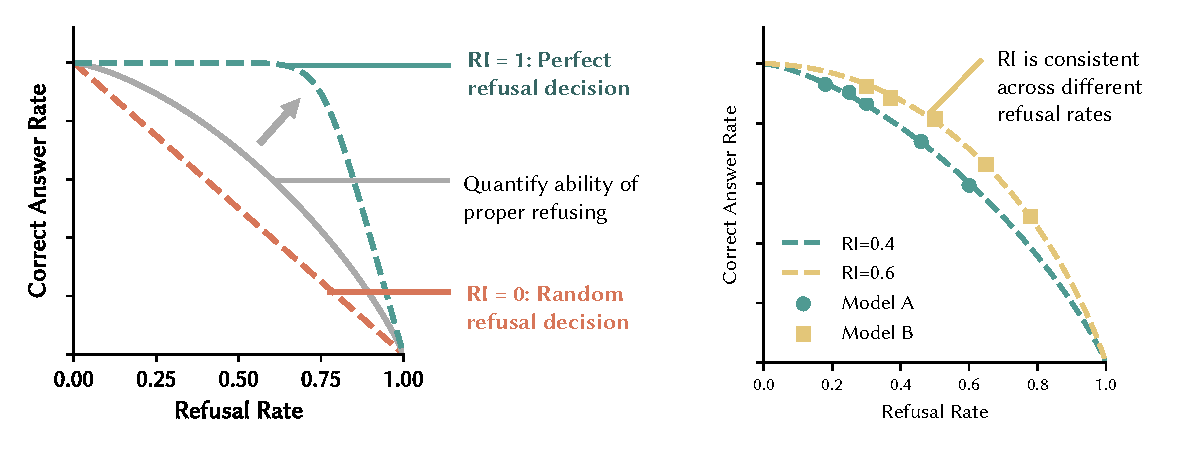
\includegraphics[width=0.95\linewidth]{Figures/RefusalIndex-Illustration.pdf}
    \vspace{-1em}
    \caption{Illustration of Refusal Index (RI). Refusal Index quantifies a model's  internal capability to refuse questions beyond its knowledge by measuring the correlation between refusal decisions and answer incorrectness. Left: Refusal Index models how the correct answer rate drops with increasing refusal rate. Right: Empirical correct answer rates for the same model at different refusal rates align with the Refusal Index. }
    \label{fig:refusal_index_illustration}
    \vspace{-1.5em}
\end{figure}

We propose a metric called the \emph{Refusal Index (RI)} to measure knowledge-aware refusal in factual tasks, which features two key properties:
\textbf{(1) accurate estimates of knowledge-aware refusal}: We formally define the Refusal Index as the Spearman correlation between refusal probabilities and error probabilities (\Secref{sec:refusal_index_method}). 
This definition is independent of refusal rate and directly targets refusal behavior, making it an unbiased measure. 
\textbf{(2) lightweight evaluation procedure}: 
Unlike previous calibration metrics that require expensive calibration processes, we only need two standard evaluation passes to compute RI, which is compatible with existing evaluation pipelines.
Specifically, we first evaluate a model on a factual question-answering dataset, collecting correct answer rates and refusal rates. 
Then, we run a second evaluation pass to regenerate answers for refused questions. 
Finally, we compute RI using the correct answer rates and refusal rates from both evaluation passes.

We perform extensive experiments and analyses to validate RI across 16 models on 5 datasets. 
We demonstrate that RI quantifies models' capability to refuse questions they do not know. 
As shown in \Figref{fig:refusal_index_illustration}, RI parameterizes the relationship between correct answer rates and refusal rates through an accuracy-refusal curve, whose convexity captures a model's ability to minimize false refusals.
This analytical model is supported by the empirical results, with consistent RI scores on the same model at different refusal rates, which align with the accuracy-refusal curve.
We also discover that RI has high agreement with established calibration metrics and provides consistent model rankings independent of a model's correctness and refusal rates. 

Beyond RI's efficacy in capturing knowledge-aware refusal, we leverage it to reveal a critical gap in current factuality evaluation: the disconnect between factual accuracy and knowledge-aware refusal capabilities. Our analysis reveals three key insights that traditional metrics overlook:
\textbf{(1) RI identifies persistent capability gaps.} While LLMs achieve high accuracy on factual tasks, their refusal behavior is unreliable. This gap remains stable across different prompting strategies and cannot be resolved by simply improving accuracy or adjusting refusal rates;
\textbf{(2) Training data and pipelines influence refusal behavior.} The model family emerges as the strongest predictor of knowledge-aware refusal ability, with certain families consistently outperforming others regardless of model scale; and
\textbf{(3) Knowledge-aware refusal is sensitive to noisy context.} Models exhibit significantly degraded refusal performance when ground truth information is unavailable in the provided context, suggesting over-reliance on contextual cues.
These findings demonstrate that RI captures an essential dimension of model reliability absent from existing factuality metrics, highlighting the need to incorporate knowledge-aware refusal measures for a more comprehensive factuality evaluation.
